\documentclass[final,hyperref={pdfpagelabels=false},xcolor=table]{beamer}
\mode<presentation>{
	\usetheme{ucb}
}
\usepackage[size=custom,width=101.6,height=76.2,scale=1.5]{beamerposter}
\usepackage{multicol}
\usepackage{graphicx}
\usepackage{textcomp}
%\usepackage{booktabs}
%\usepackage{multirow}
%\usepackage{listings}
%\usepackage{siunitx}
\usepackage{blindtext}

\graphicspath{{../figures/}}

\definecolor{ucb-pacific}{HTML}{5B6770}

\newcommand{\uT}{{\textmu}T}
\setlength{\leftmargini}{4em}

\title{Nephele: A Simple Solution for Data Replication}
\author{Joao Carreira, Howard Mao, and Nathan Pemberton}
\advisor{Randy Katz}
\institute[UC Berkeley]{\textsc{University of California, Berkeley}}

\begin{document}
\begin{frame}
\vspace{-1.5em}
\begin{columns}[t]
	\begin{column}{0.3\linewidth}
            \begin{block}{Motivation}
    As the number of nodes in distributed systems increases, failures become
    the rule, not the exception. Because of this, it is important to be able to
    recover from crashes quickly and with minimal impact on performance and
    complexity. Checkpointing and manual serialization/deserialization are both
    slow and complicated.
\end{block}

            \vspace{1ex}
            \begin{block}{RVM API}
    RVM allows the user to allocate recoverable regions of memory and
    atomically replicate changes to that memory to a remote node’s DRAM. The
    user simply identifies recovery points in their code through a
    transactional API.

    \vspace{1ex}

    \begin{tabular}{ | l | l | }
        \hline rvm\_cfg\_[create/destroy]() & \pbox{20cm}{Initialize the system \\
        and recover memory if needed} \\
        \hline rvm\_[alloc/free]() & \pbox{20cm}{Allocate a region \\
        of recoverable memory} \\
        \hline rvm\_txn\_[start/commit]() & \pbox{20cm}{Mark a point of \\
        consistency in the program} \\
        \hline rvm\_[set/get]\_usr\_data() & \pbox{20cm}{Register a pointer \\
        to your state.} \\
        \hline
    \end{tabular}
\end{block}

            \vspace{1ex}
            \begin{block}{Backends}
    Underneath the RVM layer is a remote memory backend, which handles
    communication with the remote node. The rmem layer implements basic
    functions like \texttt{malloc()}, \texttt{free()}, \texttt{put()},
    \texttt{get()}, and \texttt{commit()}. So far we have implemented two
    different backends. One uses a custom protocol based on Infiniband RDMA.
    The other uses RAMCloud, an Infiniband-based key-value store.
\end{block}

	\end{column}

	\begin{column}{0.3\linewidth}
            \begin{block}{Architecture}
    \centering
    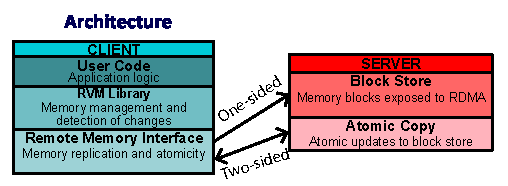
\includegraphics[width=0.9\textwidth]{lasagna.pdf}
\end{block}

	\end{column}

	\begin{column}{0.3\linewidth}
	\end{column}
\end{columns}
\end{frame}
\end{document}
